\subsection{Landmark Influence Acts Extracted from the Corpus}
\label{sec:landmarks}

Figure~\ref{fig:timeline} placed externally known events on a timeline. Figure~\ref{fig:timeline2} does the reverse: it lets the tool nominate the landmarks. For every year from 2000 to 2026 the extended corpus was queried for the highest-scoring candidate sentences written by a decision-maker of the time (the BDFL, a BDFL delegate or a Steering Council member) that carry one of the four decision-closing controversial mechanisms---unilateral, gatekeeping, exit threat or backchannel---and the top-ranked sentence was taken as the year's landmark act (1999 has too few candidates to rank). In three years a lower-ranked sentence from the top six was preferred because it is the more explicit decision act: the BDFL's ``executive decision'' on PEP~380 (2009), the delegate's acceptance of asyncio (2013) and the council's refusal to rubber-stamp (2020); the selection is otherwise mechanical. Table~\ref{tab:landmarks} lists the sentences. Below the axis, the figure stacks the share of each year's influence candidates written by each role, so that the acts can be read against who was doing the talking.

Read in sequence, the sentences trace the change in the \emph{language of decision} that the era statistics of Section~\ref{sec:rq6} only summarise. From 2001 to 2009 the landmark act is a personal pronouncement---``add a BDFL pronouncement to the PEP to end the argument'' (PEP~255), ``I'm going to make this a BDFL pronouncement; I understand your argument but I don't agree with it'' (PEP~285), ``I hereby officially reject PEP~317'', ``I am going to have to take an executive decision and override your opposition'' (PEP~380)---with the BDFL yielding to the community exactly once (``This seems to be the overwhelming feedback at this point, so I'm withdrawing my support'', PEP~363). From 2010 the acts document delegation: the BDFL appoints a ``chair of the approval process'' for PEP~3148, and from 2011 the landmark sentence is a delegate's ``as the BDFOP for PEP~3151, I hereby accept it'', ``I have decided to mark PEP~3156 accepted'', ``as BDFL-Delegate, I am officially accepting PEP~493''. The BDFL's own last acts are a rejection ``to cut this thread short'' (PEP~505, 2015), a backchannel made public (``I've been discussing this PEP offline with Victor, but he suggested we should discuss it in public instead'', PEP~540, 2017) and the resignation sentence of 2018. From 2019 the formula changes register again: acceptance ``with the unanimous backing of the rest of the Steering Council'' (PEP~581), the insistence that ``the steering council does not rubber stamp Guido's PEPs'' (PEP~622), postponement ``until after the Language Summit'' (PEP~654), ``the PEP was updated, so please consider it accepted'' (PEP~686), a delegate who ``will step down \ldots if Paul asks me'' but otherwise refuses to recuse himself (PEP~722), a council withdrawing its own PEP ``as the consensus is that the benefits doesn't justify the cost'' (PEP~758/760), and decisions that ``reflect internal discussion'' (PEP~788). The role bars tell the same story from the other side: the BDFL's share of influence candidates falls from 17\% in 2000 to under 2\% in 2018 as delegates and core developers take over the decisive sentences, and the Steering Council's share peaks at 28\% in 2022 before settling near 8\% as the council's work moves into its own meetings.

\begin{figure*}[t]
\centering
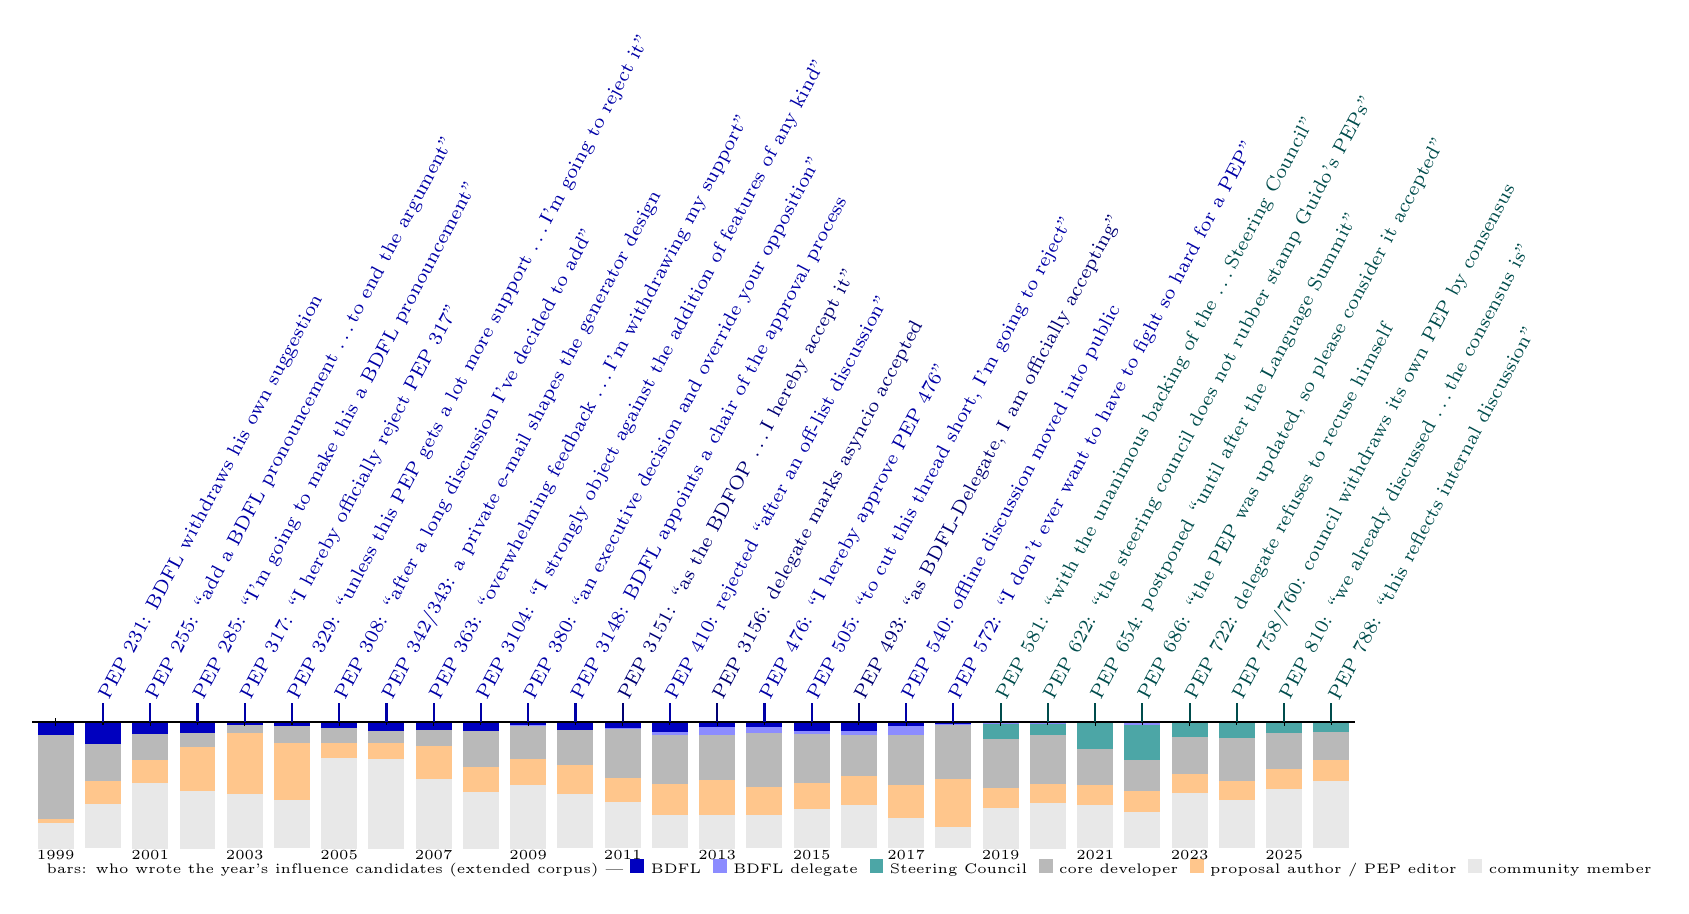
\begin{tikzpicture}[x=0.6cm, y=1cm, font=\scriptsize]
  % ---- stacked role shares of the year's influence candidates (extended corpus) ----
  % order (bottom to top): BDFL, BDFL delegate, steering council, core developer, author+editor, community
  \foreach \yr/\a/\b/\c/\d/\e/\f in {
    1999/10.0/0.0/0.0/66.3/3.8/20.0, 2000/17.2/0.0/0.0/29.2/18.4/35.2, 2001/9.2/0.0/0.0/20.9/17.9/52.1,
    2002/8.4/0.0/0.0/11.2/35.1/45.4, 2003/1.7/0.0/0.0/6.9/48.3/43.1, 2004/2.7/0.0/0.0/13.4/45.8/38.1,
    2005/4.4/0.0/0.0/11.6/12.5/71.6, 2006/6.8/0.0/0.0/9.3/12.9/71.1, 2007/6.2/0.0/0.0/12.9/26.0/55.0,
    2008/7.0/0.0/0.0/28.4/19.7/45.0, 2009/2.1/0.6/0.0/26.7/20.2/50.5, 2010/6.0/0.0/0.0/27.6/23.5/42.9,
    2011/4.2/1.2/0.0/38.8/19.0/36.8, 2012/7.5/2.4/0.0/38.7/25.0/26.3, 2013/3.9/6.1/0.0/35.7/27.7/26.7,
    2014/3.5/5.1/0.0/42.4/22.8/26.1, 2015/6.6/2.8/0.0/38.8/20.3/31.5, 2016/7.2/2.7/0.0/32.6/23.2/34.3,
    2017/3.2/7.1/0.0/39.2/26.0/24.3, 2018/1.6/0.7/0.0/42.7/37.7/16.7, 2019/0.0/1.4/11.5/38.9/16.2/32.1,
    2020/0.0/1.5/8.6/38.9/15.0/36.1, 2021/0.0/0.2/20.8/28.6/16.3/34.0, 2022/0.0/1.7/28.0/24.4/16.8/29.1,
    2023/0.0/0.4/11.3/29.4/15.2/43.7, 2024/0.0/0.2/12.1/34.5/15.0/38.2, 2025/0.0/0.6/7.8/29.0/15.1/47.5,
    2026/0.0/0.4/7.6/22.2/16.4/53.4} {
    \pgfmathsetmacro{\xl}{\yr-1999+0.12}
    \pgfmathsetmacro{\xr}{\yr-1999+0.88}
    \pgfmathsetmacro{\ya}{-\a*0.016}
    \pgfmathsetmacro{\yb}{\ya-\b*0.016}
    \pgfmathsetmacro{\yc}{\yb-\c*0.016}
    \pgfmathsetmacro{\yd}{\yc-\d*0.016}
    \pgfmathsetmacro{\ye}{\yd-\e*0.016}
    \pgfmathsetmacro{\yf}{\ye-\f*0.016}
    \fill[blue!75!black] (\xl,0) rectangle (\xr,\ya);
    \fill[blue!45] (\xl,\ya) rectangle (\xr,\yb);
    \fill[teal!70] (\xl,\yb) rectangle (\xr,\yc);
    \fill[gray!55] (\xl,\yc) rectangle (\xr,\yd);
    \fill[orange!45] (\xl,\yd) rectangle (\xr,\ye);
    \fill[gray!18] (\xl,\ye) rectangle (\xr,\yf);
  }
  \node[anchor=west, font=\tiny, align=left] at (0.1,-1.85) {bars: who wrote the year's influence candidates (extended corpus) ---
    \textcolor{blue!75!black}{\rule{5pt}{5pt}} BDFL\;
    \textcolor{blue!45}{\rule{5pt}{5pt}} BDFL delegate\;
    \textcolor{teal!70}{\rule{5pt}{5pt}} Steering Council\;
    \textcolor{gray!55}{\rule{5pt}{5pt}} core developer\;
    \textcolor{orange!45}{\rule{5pt}{5pt}} proposal author / PEP editor\;
    \textcolor{gray!18}{\rule{5pt}{5pt}} community member};
  % ---- axis and years ----
  \draw[thick] (0,0) -- (28,0);
  \foreach \yr in {1999,2001,...,2025} {
    \draw (\yr-1999+0.5,0.05) -- (\yr-1999+0.5,-0.05);
    \node[font=\tiny] at (\yr-1999+0.5,-1.68) {\yr};
  }
  \foreach \yr in {2000,2002,...,2026} { \draw (\yr-1999+0.5,0.03) -- (\yr-1999+0.5,-0.03); }
  % ---- one landmark influence act per year, nominated by the tool (Table tab:landmarks) ----
  \tikzset{bdfl/.style={blue!65!black}, dele/.style={blue!45!black}, sc/.style={teal!60!black}}
  \foreach \yr/\c/\t in {
    2000/bdfl/{PEP 231: BDFL withdraws his own suggestion},
    2001/bdfl/{PEP 255: ``add a BDFL pronouncement \ldots to end the argument''},
    2002/bdfl/{PEP 285: ``I'm going to make this a BDFL pronouncement''},
    2003/bdfl/{PEP 317: ``I hereby officially reject PEP 317''},
    2004/bdfl/{PEP 329: ``unless this PEP gets a lot more support \ldots I'm going to reject it''},
    2005/bdfl/{PEP 308: ``after a long discussion I've decided to add''},
    2006/bdfl/{PEP 342/343: a private e-mail shapes the generator design},
    2007/bdfl/{PEP 363: ``overwhelming feedback \ldots I'm withdrawing my support''},
    2008/bdfl/{PEP 3104: ``I strongly object against the addition of features of any kind''},
    2009/bdfl/{PEP 380: ``an executive decision and override your opposition''},
    2010/bdfl/{PEP 3148: BDFL appoints a chair of the approval process},
    2011/dele/{PEP 3151: ``as the BDFOP \ldots I hereby accept it''},
    2012/bdfl/{PEP 410: rejected ``after an off-list discussion''},
    2013/dele/{PEP 3156: delegate marks asyncio accepted},
    2014/bdfl/{PEP 476: ``I hereby approve PEP 476''},
    2015/bdfl/{PEP 505: ``to cut this thread short, I'm going to reject''},
    2016/dele/{PEP 493: ``as BDFL-Delegate, I am officially accepting''},
    2017/bdfl/{PEP 540: offline discussion moved into public},
    2018/bdfl/{PEP 572: ``I don't ever want to have to fight so hard for a PEP''},
    2019/sc/{PEP 581: ``with the unanimous backing of the \ldots Steering Council''},
    2020/sc/{PEP 622: ``the steering council does not rubber stamp Guido's PEPs''},
    2021/sc/{PEP 654: postponed ``until after the Language Summit''},
    2022/sc/{PEP 686: ``the PEP was updated, so please consider it accepted''},
    2023/sc/{PEP 722: delegate refuses to recuse himself},
    2024/sc/{PEP 758/760: council withdraws its own PEP by consensus},
    2025/sc/{PEP 810: ``we already discussed \ldots the consensus is''},
    2026/sc/{PEP 788: ``this reflects internal discussion''}} {
    \draw[\c, thick] (\yr-1999+0.5,0) -- (\yr-1999+0.5,0.25);
    \node[\c, rotate=62, anchor=west, inner sep=1pt] at (\yr-1999+0.5,0.27) {\t};
  }
\end{tikzpicture}
\caption{Landmark influence acts nominated by Influence Miner, 2000--2026: for each year, the highest-scoring sentence by a decision-maker of the time that carries a decision-closing mechanism (unilateral, gatekeeping, exit threat or backchannel), coloured by the author's role (dark blue: the BDFL; mid blue: a BDFL delegate; teal: a Steering Council member); full sentences in Table~\ref{tab:landmarks}. Below the axis, the share of each year's influence candidates written by each role. The sequence runs from personal pronouncements (2001--2009) through delegation (2010--2017) to the council's formulas of collective and procedural decision (2019--2026).}
\label{fig:timeline2}
\Description{A horizontal timeline from 1999 to 2026 with one short quoted sentence per year rising from the axis at an angle, coloured by whether the BDFL, a delegate or a Steering Council member wrote it, and stacked bars below the axis showing the share of influence candidates written by each role per year; the BDFL's share shrinks over time and the Steering Council's appears from 2019.}
\end{figure*}

\begin{table*}[t]
\caption{The landmark influence acts of Figure~\ref{fig:timeline2}: for each year, the highest-scoring decision-closing sentence by a decision-maker of the time in the extended corpus (score in brackets; mechanisms as labelled by the tool).}
\label{tab:landmarks}
\footnotesize
\begin{tabular}{p{0.03\textwidth}p{0.04\textwidth}p{0.14\textwidth}p{0.11\textwidth}p{0.60\textwidth}}
\toprule
Year & PEP & Author (role) & Mechanisms & Sentence \\
\midrule
2000 & 231 & van Rossum (BDFL) & exit threat & I withdraw the suggestion, and propose restricted execution instead. [2.6] \\
2001 & 255 & van Rossum (BDFL) & authority, unilateral & Tim, please add a BDFL pronouncement to the PEP to end the argument. [3.2] \\
2002 & 285 & van Rossum (BDFL) & authority, unilateral & I'm going to make this a BDFL pronouncement; I understand your argument but I don't agree with it. [4.3] \\
2003 & 317 & van Rossum (BDFL) & unilateral & I hereby officially reject PEP 317. [4.2] \\
2004 & 329 & van Rossum (BDFL) & unilateral & Also, a heads up: unless this PEP gets a lot more support from folks whose first name isn't Raymond, I'm going to reject it. [4.6] \\
2005 & 308 & van Rossum (BDFL) & compatibility, unilateral & After a long discussion I've decided to add a shortcut conditional expression to Python 2.5. [3.7] \\
2006 & 343 & van Rossum (BDFL) & backchannel & Bram Cohen pointed out in private email that, before PEP 342, there wasn't a big need for a shortcut to pass control to a ``sub-generator'' \ldots [3.7] \\
2007 & 363 & van Rossum (BDFL) & coalition, exit threat & This seems to be the overwhelming feedback at this point, so I'm withdrawing my support for the proposal. [4.4] \\
2008 & 3104 & van Rossum (BDFL) & operational, gatekeeping & I strongly object against the addition of features of *any* kind to 3.0.1, no matter whether they were promised or announced in a PEP or in the docs or on the 8 o'clock news. [4.0] \\
2009 & 380 & van Rossum (BDFL) & unilateral & Well, after thinking about it some more I think I am going to have to take an executive decision and override your opposition. :-) [2.6] \\
2010 & 3148 & van Rossum (BDFL) & unilateral & Since I really don't have the time or expertise to make a judgment on this PEP, I hereby appoint you chair of the approval process for this PEP. [3.6] \\
2011 & 3151 & Warsaw (delegate) & compatibility, unilateral & As the BDFOP for PEP 3151, I hereby accept it for inclusion into Python 3.3. [4.3] \\
2012 & 410 & van Rossum (BDFL) & authority, unilateral, backchannel & After an off-list discussion with Victor I have decided to reject PEP 410. [4.6] \\
2013 & 3156 & Pitrou (delegate) & authority, unilateral & I have decided to mark PEP 3156 accepted. [2.9] \\
2014 & 476 & van Rossum (BDFL) & unilateral & I see no reason to hold up this PEP's approval any longer, so I hereby approve PEP 476. [4.0] \\
2015 & 505 & van Rossum (BDFL) & unilateral & Just to cut this thread short, I'm going to reject PEP 505, because ? is just too ugly to add to Python IMO. [4.2] \\
2016 & 493 & Warsaw (delegate) & authority, unilateral & As BDFL-Delegate, I am officially accepting PEP 493. [2.9] \\
2017 & 540 & van Rossum (BDFL) & backchannel & I've been discussing this PEP offline with Victor, but he suggested we should discuss it in public instead. [4.2] \\
2018 & 572 & van Rossum (BDFL) & coalition, exit threat & Now that PEP 572 is done, I don't ever want to have to fight so hard for a PEP and find that so many people despise my decisions. [4.4] \\
2019 & 581 & Warsaw (SC) & authority, coalition, unilateral & As the BDFL-Delegate for PEP 581, and with the unanimous backing of the rest of the Steering Council, I hereby Accept this PEP. [4.6] \\
2020 & 622 & Cannon (SC) & authority, incivility, backchannel & I'm trying to not take that as an insult, but I will say the steering council does not rubber stamp Guido's PEPs. [2.7] \\
2021 & 654 & Galindo Salgado (SC) & tactical, authority, backchannel & The Steering Council discussed PEP 654: Exception Groups and except* \ldots deciding to postpone the PEP to 3.11, and postpone their decision for 3.11 until after the Language Summit. [3.6] \\
2022 & 686 & Viktorin (SC) & unilateral & The PEP was updated, so please consider it accepted. [4.0] \\
2023 & 722 & Cannon (SC) & authority, exit threat & I will step down as PEP delegate if Paul asks me, but otherwise I disagree with your reasoning as to why I shouldn't be the PEP delegate in this situation, and so I have no plans to recuse myself. [4.2] \\
2024 & 758/760 & Galindo Salgado (SC) & economic, coalition, exit threat & Update: We have decided to withdraw the PEP as the consensus is that the benefits doesn't justify the cost. [3.6] \\
2025 & 810 & Galindo Salgado (SC) & coalition, backchannel, procedural & We already discussed some version of this early in the discussion and the consensus is that \texttt{mod.\_\_dict\_\_} should not reify. [3.5] \\
2026 & 788 & Na (SC) & operational, backchannel & This reflects internal discussion that, if the PEP is officially approved, the implementer should have enough time to proceed with the implementation before the beta cutoff (May 5). [4.1] \\
\bottomrule
\end{tabular}
\end{table*}

